%%%%%%%%%%%%%%%%%%%%%%%%%%%%%%%%%%%%%%%%%%%%%%%%%%%%%%%%%%%%%%%%%%%%%%%%%%%%%%%%
%% MASTER'S THESIS                                                            %%
%%                                                                            %% 
%% Title (en): Multi-Agent Systems and Organizations                          %%
%% Title (cs): Multiagentní systémy a organizace                              %%
%%                                                                            %%
%% Author: Bc. Lukáš Kúdela                                                   %%
%% Supervisor: Prof. RNDr. Petr Štěpánek, DrSc.                               %%
%%                                                                            %%
%% Academic year: 2011/2012                                                   %%
%%%%%%%%%%%%%%%%%%%%%%%%%%%%%%%%%%%%%%%%%%%%%%%%%%%%%%%%%%%%%%%%%%%%%%%%%%%%%%%%

\chapter{Platform-Independent Metamodel---Thespian}

% Chapter intro
In this chapter, we will present our platform-independent metamodel for modelling organizations in MASs---\textit{Thespian}.
\textit{Thespian} is one of our two contributions to the field, the other one being \textit{Thespian4Jade}.

% Thespian - defnition
\textit{Thespian} is a metamodel to which platform-independent models of organizations in MASs must conform; more precisely, it is a model\footnote{Recall that a metamodel is a kind of model.} representing a modelling language \footnote{When can call this language the \textit{Thespian modelling language}.} to which platform-independent models of organizations in MASs must conform.

% Thespian name inspiration - Thespis of Icaria
The metamodel is named after \textit{Thespis of Icaria} (present-day Dionysos, Greece), who lived in the 6th century BC and, according to certain Ancient Greece sources and especially Aristotle, was the first person ever to appear on stage as an actor playing a character in a play (instead of speaking as themselves) \cite{Wikipedia-Thespis}.

% Thespian inspiration - Aalaadin, O&P, PIM4Agents and powerJade
The design of \textit{Thespian} is inspired, to a greater or lesser degree, by all four metamodels introduced in the previous chapter.
% Aaalaadin
Similarly to \textit{Aalaadin}, its static model can be partitioned into a \textit{run-time model} and \textit{design-time model} (called \textit{core model} and \textit{methodological model} respectively in \textit{Aalaadin}.)
% O&P
Like \textit{O\&P}, it can be used to model \textit{holonic} MASs\footnote{A \textit{holonic} MAS is a MAS where agents are \textit{holons}---simultaneously a \textit{whole} and a \textit{part}. This means that the agents in a holonic MAS can not only form aggregations, but these aggregations are full-fledged agents; in particular, they can form other aggregations and so on. An \textit{object} from OOP is another example of a holon.}.
% PIM4Agents
Similarly to \textit{PIM4Agents}, its static model contains concepts for modelling protocols and messages exchanged in these protocols. Overall, \textit{PIM4Agents} has had the least influence on \textit{Thespian} from all four metamodels.
% powerJade
And like \textit{powerJade}, it can be used to represent role \textit{competences} and \textit{responsibilities} (called \textit{powers} and \textit{requirements} respectively in \textit{powerJade}).
Furthermore, \textit{Thespian's} dynamic model also makes a distinction between \textit{enacting} a role and actually \textit{activating} it.
All in all, \textit{powerJade} has had the greatest influence on \textit{Thespian} from all four metamodels.

% Static & dynamic models
The metamodel encompasses
\begin{itemize}
	\item a \textit{static model} for modelling static (structural) aspects of organizations, and
	\item a \textit{dynamic model} for modelling their dynamic (behavioural) aspect.
\end{itemize}
In the following two sections, we will introduce both models in detail.

%%%%%%%%%%%%%%%%%%%%%%%%%%%%%%%%%%%%%%%%%%%%%%%%%%%%%%%%%%%%%%%%%%%%%%%%%%%%%%%%
%% MASTER'S THESIS                                                            %%
%%                                                                            %% 
%% Title (en): Multi-Agent Systems and Organizations                          %%
%% Title (cs): Multiagentní systémy a organizace                              %%
%%                                                                            %%
%% Author: Bc. Lukáš Kúdela                                                   %%
%% Supervisor: Prof. RNDr. Petr Štěpánek, DrSc.                               %%
%%                                                                            %%
%% Academic year: 2011/2012                                                   %%
%%%%%%%%%%%%%%%%%%%%%%%%%%%%%%%%%%%%%%%%%%%%%%%%%%%%%%%%%%%%%%%%%%%%%%%%%%%%%%%%

\section{Static Metamodel}

The static \textit{Thespian} metamodel is used to model static (structural) aspects of OCMAS like:
\begin{itemize}
	\item an organization's role structure and protocols,
	\item a role's competences and responsibilities or
	\item a player's capabilities.
\end{itemize}

%%%%%%%%%%%%%%%%%%%%%%%%%%%%%%%%%%%%%%%%%%%%%%%%%%%%%%%%%%%%%%%%%%%%%%%%%%%%%%%%
\subsection{Organization Metamodel}

% Organization metamodel - usage
The Organization metamodel (figure~\ref{figure:thespian-organization-metamodel}) contains concepts whose instances model organizations and roles with their competences and responsibilities.

\subsubsection*{Organization and Organization Type}

% Type-token distinction - organization
To enable the type-token distinction, \textit{Thespian} contains concepts for modelling both an \textit{organization type} and an \textit{organization token}: \textit{Organization type} and \textit{Organization}.

% Organization
\textit{Organization} (also called \textit{Organization instance}) is an actual organization in a running MAS; it is a run-time entity.
% Organization - state
It is classified by an \textit{Organization type} which specifies its role structure.
% Organization - note
Note that despite an organization being a run-time entity, it can be declared at design-time, created at MAS start-up and destroyed at MAS shut-down.

% Organization type
\textit{Organization type} (also called \textit{Organization class}) is a class of organizations sharing the same role structure; it is a design-time entity.
% Organization type - state
It contains a set of \textit{Roles} defining its role structure.
% Organization type - behaviour
It can be instantiated to yield an \textit{Organization}. 

\subsubsection*{Role and Position}

% Type-token distinction - role
\textit{Thespian} contains concepts for modelling both an \textit{role type} and \textit{role token} to enable the type-token distinction: \textit{Role} and \textit{Position}.

% Role
\textit{Role} is a role specification within an organization; it is a design-time entity.
% Role - state
It has a set of \textit{Competences} and a set of \textit{Responsibilities} defining its function in its containing \textit{Organization type} and multiplicity differentiating between a \textit{single role})---one that can not be played by more than one \textit{Player} in an \textit{Organization}---and a \textit{multiple role}---one that can.
Currently, neither \textit{Thespian} not \textit{Thespian4Jade} support differentiating between a \textit{mandatory role}---one that has to be played at all times---and an \textit{optional role}---one that does not have to be.

% Position
A \textit{Position} (sometimes called \textit{Role instance}) is a role realization within an actual organization; it is a run-time entity.
% Position - state
It is a realization of \textit{Role} which specifies its competences
It belongs to an \textit{Organization} and is played by a \textit{Player}.
% Position - note
Note that a \textit{Position} is usually not declared at design-time; it is created when an \textit{Player} starts playing a role in an \textit{Organization} and destroyed when that \textit{Player} stops doing so.

\subsubsection*{Competence and Responsibility}

Let us consider a player playing a role.
As a result of playing the role, the player gains competences a responsibilities associated with that role.

% Competence
\textit{Competence} is an operation a player playing a role \textit{can} can execute as a result of playing that role; it is a design-time entity.
% Competence - state
A \textit{Competence} can require an argument from a player after its invocation (but before its execution), in which case the argument type (a Java type) has to be specified.
Also it can provide a return value to the player after its execution, in which case the return value type (a Java type) has to be specified.

% Figure: Thespian - Organization metamodel
\begin{figure}[ht]
	\centering
	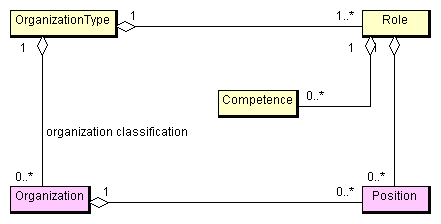
\includegraphics[width=0.8\textwidth]{images/thespian/organization-metamodel.png}
	\caption{The Organization metamodel}
	\label{figure:thespian-organization-metamodel}
\end{figure}

%%%%%%%%%%%%%%%%%%%%%%%%%%%%%%%%%%%%%%%%%%%%%%%%%%%%%%%%%%%%%%%%%%%%%%%%%%%%%%%%
\subsection{Player Metamodel}

% Player metamodel - usage
The Player metamodel (figure~\ref{figure:thespian-player-metamodel}) contains constructs for modelling players and their responsibilities.

\subsubsection*{Player and Player Type}

% Type-token distinction - player
To facilitate the type-token distinction, \textit{Thespian} contains concepts for modelling both a \textit{player type} and a \textit{player token}: \textit{Player type} and \textit{Player}.

% Player
\textit{Player} is an actual player in a running MAS; it is a run-time entity.
% Player - state
It is classified by a player type which specifies its responsibilities.
% Player - note
Note that despite a player being a run-time entity, it has to be declared at design-time, created at MAS start-up and destroyed at MAS shut-down.

% Player type
\textit{Player type} (also called \textit{Player class})is a class of players sharing the same characteristics, namely responsibilities; it is a design-time entity.
% Player type - state
It has a set of responsibilities defining its capabilities when playing a role.
% Player type - behaviour
It can be instantiated to yield a player. 

\subsubsection*{Responsibility}

% Responsibility
\textit{Responsibility}is an operation a player playing a role \textit{must} execute as a result of playing that role; it is a design-time entity. 
% Responsibility - state
A \textit{Responsibility} can provide an argument to a player after its invocation (but before its execution), in which case the argument type (a Java type) has to be specified.
Also it can request a return value from the player after its execution, in which case the return value type (a Java type) has to be specified.

% Figure: Thespian - Player metamodel
\begin{figure}[ht]
	\centering
	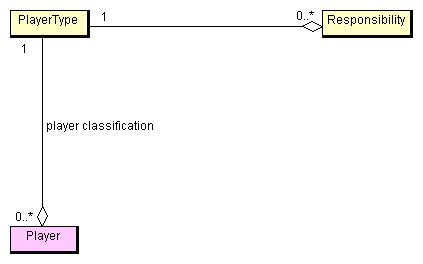
\includegraphics[width=0.4\textwidth]{images/thespian/player-metamodel.png}
	\caption{The Player metamodel}
	\label{figure:thespian-player-metamodel}
\end{figure}

%%%%%%%%%%%%%%%%%%%%%%%%%%%%%%%%%%%%%%%%%%%%%%%%%%%%%%%%%%%%%%%%%%%%%%%%%%%%%%%%
\subsection{Protocol Metamodel}

% Protocol metamodel - usage
The Protocol metamodel (figure~\ref{figure:thespian-protocol-metamodel}) contains abstractions whose instances represent interaction protocols between a player and an organization or role, and among roles themselves.

\subsubsection*{Protocol}

% Protocol
An \textit{Interaction protocol} is an institutionalized pattern of interaction (communication) between two or more roles within an organization; it is a design-time entity modelled by the \textsc{Protocol} class.
It defines parties involved in the interaction and messages exchanged in the communication.

% Scenario
A realization of an interaction protocol is an \textit{Interaction scenario}---a sequence of actions performed (messages exchanged) by two or more roles within an organization; a scenario is a purely run-time entity.
In other words, a protocol is a framework and a scenario (is) one of its possible instantiations.
Since scenarios are usually not explicitly modelled\footnote{Scenarios can be explicitly modelled in snapshots.}, \textit{Thespian} does not contain the concept of an \textit{Interaction scenario}.

% Type-token distinction - protocol
The theme of type-token distinction is at play here: instances of \textit{Protocol} model \textit{protocol types} and instances of \textit{Scenario} represent \textit{protocol tokens}.

\subsubsection*{Party}

% Party - definition
A \textit{Party} is a role involved in a protocol; it is a design-time entity modelled by the \textsc{Party} abstract class.
A relationship between roles and protocols is a many-to-many one; a role can participate in multiple protocols and at least two different roles have to take part in a protocol; a party is a reification (embodiment) of this relationship.
% Initiator party & Responder party
A \textit{Party} is either an \textit{Initiator party}---one that initiates the protocol---or a \textit{Responder party}---one that responds to the initiated protocol. These two concepts are modelled by two concrete classes: \textsc{InitiatorParty} and \textsl{ResponderParty} respectively.

\subsubsection*{Message}

A \textit{Message} is a piece of information exchanged between two parties in a protocol; it is a design-time entity modelled by the \textsc{Message} class.

% Figure: Thespian - Protocol metamodel
\begin{figure}[ht]
	\centering
	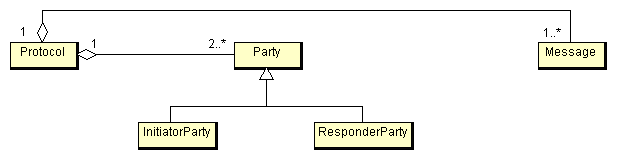
\includegraphics[width=0.8\textwidth]{images/thespian/protocol-metamodel.png}
	\caption{The Protocol metamodel}
	\label{figure:thespian-protocol-metamodel}
\end{figure}

%%%%%%%%%%%%%%%%%%%%%%%%%%%%%%%%%%%%%%%%%%%%%%%%%%%%%%%%%%%%%%%%%%%%%%%%%%%%%%%%
\subsection{Compile-Time Metamodel}	

% Design-time metamodel - usage
The Design-time metamodel contains concepts whose instances model the design-time MAS entities.
These entities, as their name suggests, are created and/or modified at design-time by the MAS designer, and they constitute the MAS specification (see this chapter's introduction).
The models of MAS specifications are also called \textit{static MAS models}.

% Figure: Thespian - Compie-time metamodel
\begin{figure}[ht]
	\centering
	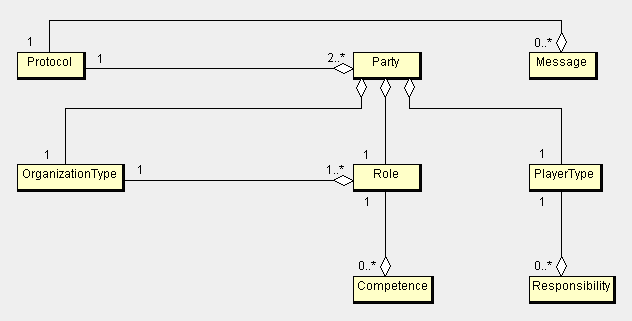
\includegraphics[width=0.8\textwidth]{images/thespian/compile-time-metamodel.png}
	\caption{The Compile-time metamodel}
	\label{figure:thespian-static-metamodel}
\end{figure}

%%%%%%%%%%%%%%%%%%%%%%%%%%%%%%%%%%%%%%%%%%%%%%%%%%%%%%%%%%%%%%%%%%%%%%%%%%%%%%%%
\subsection{Run-Time Metamodel}

% Run-time metamodel - usage
The Run-time metamodel contains constructs that model the run-time MAS entities.
These entities, as their name implies, are created and/or modified at run-time by the MAS itself, and they make up the MAS manifestation (see this chapter's introduction).
They models of MAS manifestations are also referred to as \textit{dynamic MAS models} or \textit{MAS snapshots}.

% Figure: Thespian - Run-time metamodel
\begin{figure}[ht]
	\centering
	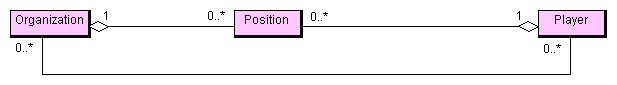
\includegraphics[width=0.8\textwidth]{images/thespian/run-time-metamodel.png}
	\caption{The Run-time metamodel}
	\label{figure:thespian-dynamic-metamodel}
\end{figure}

%%%%%%%%%%%%%%%%%%%%%%%%%%%%%%%%%%%%%%%%%%%%%%%%%%%%%%%%%%%%%%%%%%%%%%%%%%%%%%%%
\subsection{Integrated Metamodel}

Figure~\ref{figure:thespian-integrated-metamodel} shows the integrated \textit{Thespian} metamodel.

% Key property of Thespian - no association between Role and Player type
We would like to emphasize what we perceive as key property of \textit{Thespian}: there is no association between \textit{Role} and \textit{Player type}, no link between a specific role and a particular player type.
This means that there is no design-time dependency between roles and player types; all connections arise at run-time and happen between positions and players.

% Figure: Thespian integrated metamodel
\begin{figure}[ht]
	\centering
	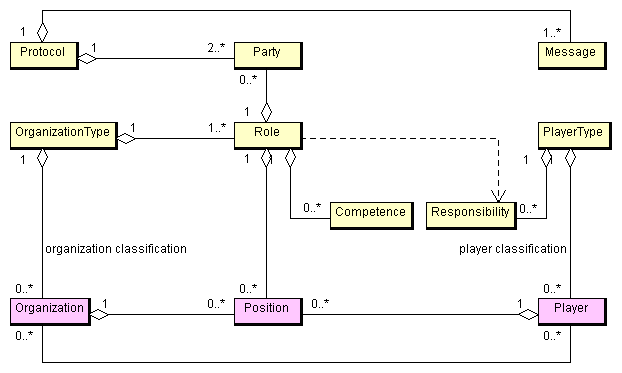
\includegraphics[width=0.8\textwidth]{images/thespian/thespian-metamodel.png}
	\caption{The Integrated metamodel}
	\label{figure:thespian-integrated-metamodel}
\end{figure}

%%%%%%%%%%%%%%%%%%%%%%%%%%%%%%%%%%%%%%%%%%%%%%%%%%%%%%%%%%%%%%%%%%%%%%%%%%%%%%%%
%% MASTER'S THESIS                                                            %%
%%                                                                            %% 
%% Title (en): Multi-Agent Systems and Organizations                          %%
%% Title (cs): Multiagentní systémy a organizace                              %%
%%                                                                            %%
%% Author: Bc. Lukáš Kúdela                                                   %%
%% Supervisor: Prof. RNDr. Petr Štěpánek, DrSc.                               %%
%%                                                                            %%
%% Academic year: 2011/2012                                                   %%
%%%%%%%%%%%%%%%%%%%%%%%%%%%%%%%%%%%%%%%%%%%%%%%%%%%%%%%%%%%%%%%%%%%%%%%%%%%%%%%%

\section{Dynamic Metamodel}

The dynamic Thespian metamodel is used to model dynamic (behavioural) aspects of OCMAS like:
\begin{itemize}
	\item players playing roles within organizations,
	\item players exercising their roles' competences and fulfilling their roles' responsibilities, or
	\item players subscribing to organization events, or
	\item organizations publishing events.
\end{itemize}

%%%%%%%%%%%%%%%%%%%%%%%%%%%%%%%%%%%%%%%%%%%%%%%%%%%%%%%%%%%%%%%%%%%%%%%%%%%%%%%%
\subsection{Player and Organization Interaction}

% Organization protocols
A player and an organization interact through four protocols: \textit{Enact role}, \textit{Deact role}, \textit{Subscribe to event} and \textit{Publish event}.

%%%%%%%%%%%%%%%%%%%%%%%%%%%%%%%%%%%%%%%%%%%%%%%%%%%%%%%%%%%%%%%%%%%%%%%%%%%%%%%%
\subsubsection{Enacting a Role}

% Figure: 'Enact role' protocol
\begin{figure}[ht]
	\centering
	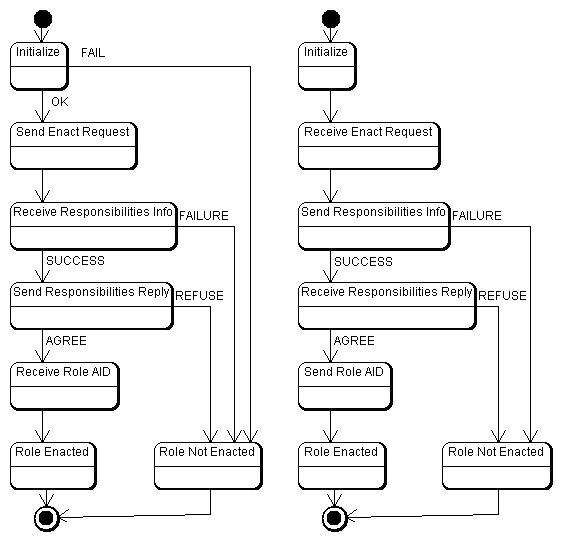
\includegraphics[width=0.8\textwidth]{images/thespian/enact-role-protocol.png}
	\caption{The \textit{Enact role} protocol}
	\label{figure:thespian-enact-role-protocol}
\end{figure}

% 'Enact a role in an organization' - definition
To \textit{enact} a role in an organization means to assume a in an organization.
% Restrictions
Naturally, only a non-enacted or multiple role can be enacted; more precisely, a role can only be enacted in a concrete organization in which it is not already enacted by any player or is defined as a multiple role.
% Protocol
A player who wants to enact a role in an organization, initiates the \textit{Enact role} protocol with that organization.

% 'Enact role' protocol - definition
The \textit{Enact role} protocol consists of the following steps:
\begin{enumerate}
	% 1
	\item The player sends an \textit{Enact role request} message to the organization containing the name of the role it wants to enact.
	% 2	
	\item The organization receives the request message and sends back either
	\begin{itemize}
		% SUCCESS
		\item a \textit{Required Responsibilities} message listing the role's responsibilities if such role exists and can be enacted, i.e. if it is not enacted by any player or is defined as a multiple role, or
		% Failure
		\item a \textit{Failure} message otherwise. 
	\end{itemize}
	% 3	
	\item Upon receiving a \textit{Required Responsibilities} message, the player then determines if it has the required capabilities to fulfil the role's responsibilities and replies either with
	\begin{itemize}
		% AGREE		
		\item an \textit{Agree} message if it has the capabilities, or
		% REFUSE
		\item a \textit{Refuse} message otherwise.
	\end{itemize}
	% 4
	\item Upon receiving an \textit{Agree} message, the organization creates a position and sends a \textit{Role AID} message containing its AID to the player.
	The organization then ends its part in the protocol.
	% 5
	\item The player receives the \textit{Role AID} message and ends its part in the protocol.
\end{enumerate}


%%%%%%%%%%%%%%%%%%%%%%%%%%%%%%%%%%%%%%%%%%%%%%%%%%%%%%%%%%%%%%%%%%%%%%%%%%%%%%%%
\subsubsection{Deacting a Role}

% Figure: 'Deact role' protocol
\begin{figure}[ht]
	\centering
	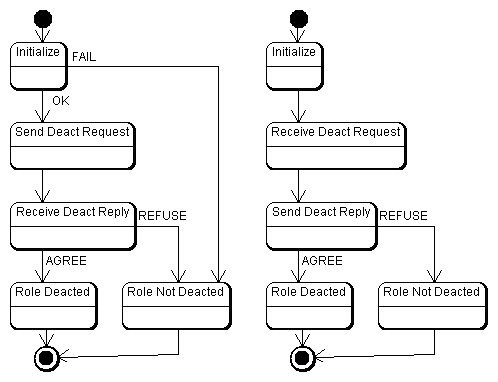
\includegraphics[width=0.8\textwidth]{images/thespian/deact-role-protocol.png}
	\caption{The \textit{Deact role} protocol}
	\label{figure:thespian-deact-role-protocol}
\end{figure}

% 'Deact a role in an organization' - definition
To \textit{deact}
\footnote{The word `deact' does not exist in the English language, it is a made-up word.}
a role in an organization means to relinquish a role in an organization.
% Restrictions
Naturally, only an enacted and inactive (see section~\ref{section:activating-a-role} for details) role can be deacted; more precisely, a role can only be deacted in a concrete organization in which it is enacted by the player and inactive.
% Protocol
A player who wants to deact a role in an organization, initiates the \textit{Deact role} protocol with that organization.

% 'Deact role' protocol - definition
The following steps comprise the \textit{Deact role} protocol:
\begin{enumerate}
	% 1
	\item The player sends a \textit{Deact role request} message to the organization containing the name of the role it wants to enact.
	% 2	
	\item The organization receives the request message and sends back either
	\begin{itemize}
		% AGREE
		\item an \textit{Agree} message if the role exists and can be deacted, i.e. if it is enacted by the player and inactive, or
		% REFUSE
		\item a \textit{Refuse} message otherwise. 
	\end{itemize}
	The organization then ends its part in the protocol.
	% 3
	\item The player receives the reply message and ends its part in the protocol.
\end{enumerate}

%%%%%%%%%%%%%%%%%%%%%%%%%%%%%%%%%%%%%%%%%%%%%%%%%%%%%%%%%%%%%%%%%%%%%%%%%%%%%%%%
\subsubsection{Subscribing to an Event}

% Figure: 'Subscribe to event' protocol
\begin{figure}[ht]
	\centering
	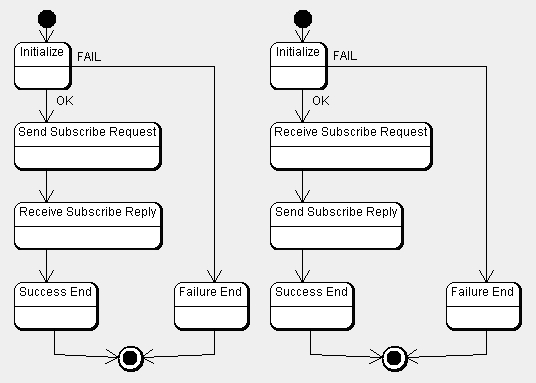
\includegraphics[width=0.8\textwidth]{images/thespian/subscribe-to-event-protocol.png}
	\caption{The \textit{Subscribe to event} protocol}
	\label{figure:thespian-subscribe-to-event-protocol}
\end{figure}

% 'Subscribe to an event in an organization' - definition
Subscribing to an event in an organization means to be notified of an event in an organization.
A player can subscribe to the \textit{role enacted}, \textit{role deacted}, \textit{role activated} and \textit{role deactivated} events raised when a role is enacted, deacted, activated and deactivated respectively.
% Restrictions
Naturally, only an employed player can subscribe to an event; more precisely, an event can only be subscribed to in a concrete organization in which the player enacts a role.
% Protocol
A player who wants subscribe to an event in an organization, initiates the \textit{Subscribe to event} protocol with that organization.

% 'Subscribe to event' protocol - definition
The \textit{Subscribe to event} protocol consists of the following steps:
\begin{enumerate}
	% 1
	\item The player sends a \textit{Subscribe to event request} message containing the name of the role it wants to enact to the organization.
	% 2	
	\item The organization receives the request message and immediately terminates if the message comes from a player that is not employed by that organization.
	If the message comes from a player employed in that organization, it sends back either
	\begin{itemize}
		% AGREE
		\item an \textit{Agree} message if the event exists, or
		% REFUSE
		\item a \textit{Refuse} message otherwise. 
	\end{itemize}
	The organization then ends its part in the protocol.
	% 3
	\item The player receives the reply message and ends its part in the protocol.
\end{enumerate}

%%%%%%%%%%%%%%%%%%%%%%%%%%%%%%%%%%%%%%%%%%%%%%%%%%%%%%%%%%%%%%%%%%%%%%%%%%%%%%%%
\subsubsection{Publishing an Event}

% Figure: 'Publish event' protocol
\begin{figure}[ht]
	\centering
	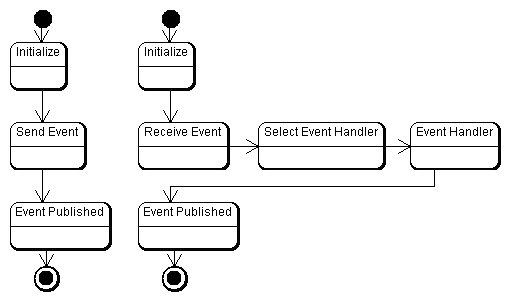
\includegraphics[width=0.8\textwidth]{images/thespian/publish-event-protocol.png}
	\caption{The \textit{Publish event} protocol}
	\label{figure:thespian-publish-event-protocol}
\end{figure}

% 'Publishing an event to subscribed players' - definition
To publish an event to its subscribers means to notify the players subscribed to an event of that event occurring.
% Restrictions
% - none
% Protocol
An organization that wants publish an event to its subscribers, initiates the \textit{Publish event} protocol with the event subscribers.

% 'Publish event' protocol - definition
The following steps comprise the \textit{Publish event} protocol:
\begin{enumerate}
	% 1	
	\item The organization sends an \textit{Event} message containing the name of the event and its argument to the event subscribers.
	The organization then ends its part in the protocol.
	% 2
	\item A subscriber receives the message and handles the event.
	The subscriber then ends its part in the protocol.
\end{enumerate}

%%%%%%%%%%%%%%%%%%%%%%%%%%%%%%%%%%%%%%%%%%%%%%%%%%%%%%%%%%%%%%%%%%%%%%%%%%%%%%%%
\subsection{Player and Role Interaction}

% Role protocols
A player and a role interact via four protocols: \textit{Activate role}, \textit{Deactivate role}, \textit{Invoke competence} and \textit{Invoke responsibility}.

%%%%%%%%%%%%%%%%%%%%%%%%%%%%%%%%%%%%%%%%%%%%%%%%%%%%%%%%%%%%%%%%%%%%%%%%%%%%%%%%
\subsubsection{Activating a Role}
\label{section:activating-a-role}

% Figure: 'Activate role' protocol
\begin{figure}[ht]
	\centering
	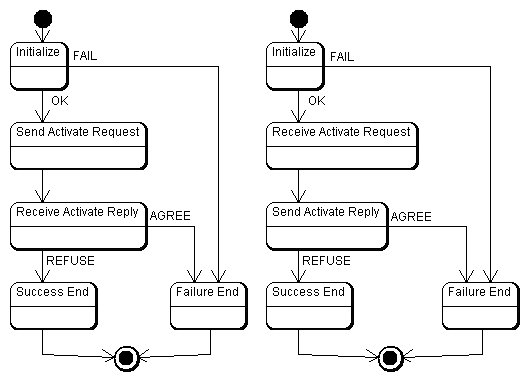
\includegraphics[width=0.8\textwidth]{images/thespian/activate-role-protocol.png}
	\caption{The \textit{Activate role} protocol}
	\label{figure:thespian-activate-role-protocol}
\end{figure}

% 'Activate a role' - definition
To \textit{activate} a role
\footnote{More precisely, what is activated is a position -- a concrete instantiation of a role in a specific organization enacted by the activating player.}
means to begin playing a role, i.e. start exercising its competences and fulfilling its responsibilities.
% Restrictions
Naturally, only an enacted and inactive role can be activated; more precisely, a role can only be activated in a concrete organization in which it is already enacted by the player and inactive.
Furthermore, a player may activate only one role (in all concrete organizations) at a time.
% Protocol
A player who wants to activate a role, initiates the \textit{Activate role} protocol with that role.

% 'Activate role' protocol - definition
The \textit{Activate role} protocol consists of the following steps:
\begin{enumerate}
	% 1
	\item The player sends a \textit{Activate role} request message to the role.
	% 2	
	\item The role receives the request message and immediately terminates if the message comes from anyone else than its player.
	If the message comes from its enacting player, it sends back either
	\begin{itemize}
		% AGREE
		\item an \textit{Agree} message if the role can be activated, i.e. it is inactive, and the player does not have any other active role in the role's organization.
		% REFUSE
		\item a \textit{Refuse} message otherwise. 
	\end{itemize}
	The role then ends its part in the protocol.
	% 3
	\item The player receives the reply message and ends its part in the protocol.
\end{enumerate}

%%%%%%%%%%%%%%%%%%%%%%%%%%%%%%%%%%%%%%%%%%%%%%%%%%%%%%%%%%%%%%%%%%%%%%%%%%%%%%%%
\subsubsection{Deactivating a Role}

% Figure: 'Deactivate role' protocol
\begin{figure}[ht]
	\centering
	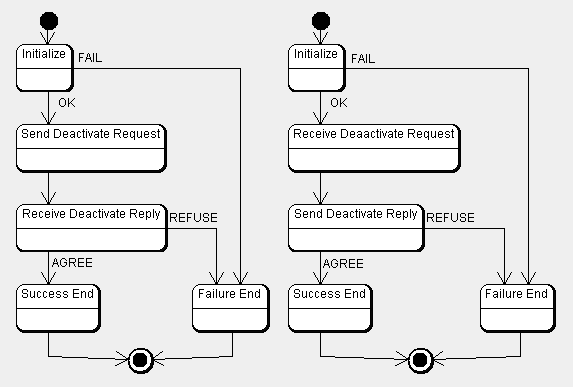
\includegraphics[width=0.8\textwidth]{images/thespian/deactivate-role-protocol.png}
	\caption{The \textit{Deactivate role} protocol}
	\label{figure:thespian-deactivate-role-protocol}
\end{figure}

% 'Deactivating a role' - definition
To \textit{deactivate} a role (more precisely, a position) means to stop playing a role, i.e. stop exercising its competences and fulfilling its responsibilities.
% Restrictions
Naturally, only an enacted and active role can be deactivated; more precisely, a role can only be deacted in a concrete organization in which it is enacted by the player and active.
% Protocol
A player who wants to deactivate a role, initiates the \textit{Deactivate role} protocol with that role.

% 'Deactiavte role' protocol - definition
The following steps comprise the \textit{Deactivate role} protocol:
\begin{enumerate}
	% 1
	\item The player sends a \textit{Deactivate role} request message to the role.
	% 2	
	\item The role receives the request message and immediately terminates if the message comes from anyone else than its player.
	If the message comes its enacting player, it sends back either
	\begin{itemize}
		% AGREE
		\item an \textit{Agree} message if the role can be deactivated, i.e. it is active, or
		% REFUSE
		\item a \textit{Refuse} message otherwise. 
	\end{itemize}
	The role then ends its part in the protocol.
	% 3
	\item The player receives the reply message and ends its part in the protocol.
\end{enumerate}

%%%%%%%%%%%%%%%%%%%%%%%%%%%%%%%%%%%%%%%%%%%%%%%%%%%%%%%%%%%%%%%%%%%%%%%%%%%%%%%%
\subsubsection{Invoking a Competence}

% Figure: 'Invoke competence' protocol
\begin{figure}[ht]
	\centering
	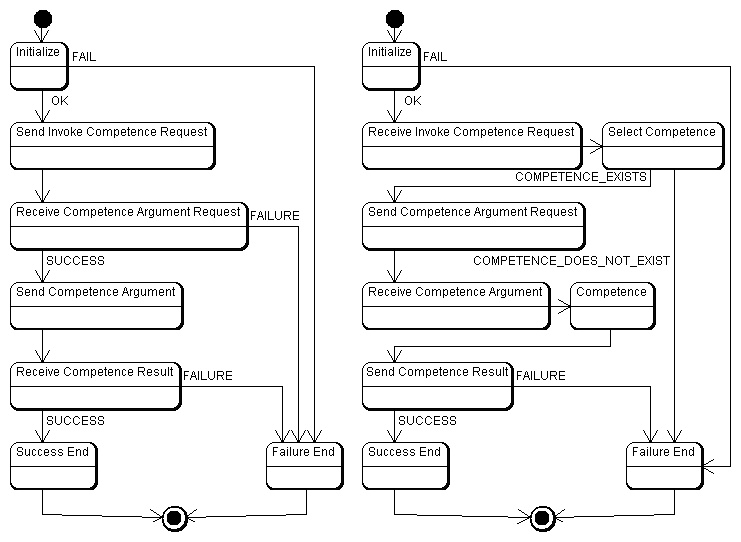
\includegraphics[width=0.8\textwidth]{images/thespian/invoke-competence-protocol.png}
	\caption{The \textit{Invoke competence} protocol}
	\label{figure:thespian-invoke-competence-protocol}
\end{figure}

% 'Invoke a competence on a role' - definition
Invoking a competence on a role (more precisely, a position) happens when a player calls upon its active role to exercise a competence.
% Restrictions
Note that a competence can only be invoked on an active role.
% Protocol
A player who wants to invoke a competence on a role, initiates the \textit{Invoke competence} protocol with that role.

% 'Invoke competence' protocol - definition
The \textit{Invoke competence} protocol consists of the following steps:
\begin{enumerate}
	% 1	
	\item The player sends an \textit{Invoke competence request} request to the role containing the name of the competence to invoke.
	% 2
	\item The role receives the request message and immediately terminates if the message comes from anyone else than its player or it is not active.
	If, on the other hand, the message comes from its player and it is active, it sends back 
	\begin{itemize}
		% SUCCES		
		\item a \textit{Competence argument request} message asking the player to provide the competence argument if the competence exists, or
		% FAILURE
		\item a \textit{Failure} message otherwise. 
	\end{itemize}
	% 3	
	\item Upon receiving the \textit{Competence argument request} message, the player sends the \textit{Competence argument} message carrying the competence argument.
	% 4
	\item The role receives the competence argument and executes the competence and sends back either
	\begin{itemize}
		% SUCCESS
		\item either a \textit{Competence result} message carrying the competence result in case the competence executed successfully, or
		\item a \textit{Failure} message otherwise.
	\end{itemize}
	The role then ends its part in the protocol.
	% 5
	\item The player receives the reply message and ends its part in the protocol.
\end{enumerate}

%%%%%%%%%%%%%%%%%%%%%%%%%%%%%%%%%%%%%%%%%%%%%%%%%%%%%%%%%%%%%%%%%%%%%%%%%%%%%%%%
\subsubsection{Invoking a Responsibility}

% Figure: 'Invoke responsibility' protocol
\begin{figure}[ht]
	\centering
	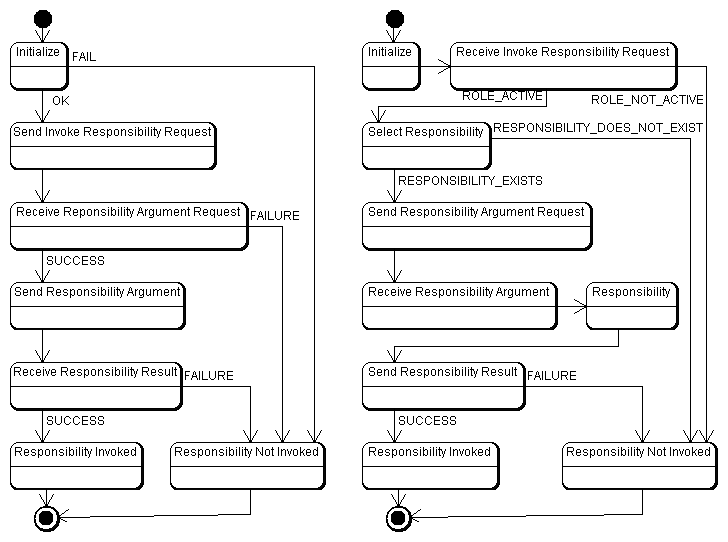
\includegraphics[width=0.8\textwidth]{images/thespian/invoke-responsibility-protocol.png}
	\caption{The \textit{Invoke responsibility} protocol}
	\label{figure:thespian-invoke-responsibility-protocol}
\end{figure}

% 'Invoke a responsibility on a player' - definition
Invoke a responsibility on a player happens when a role (more precisely, a position) calls upon its player to fulfil a responsibility.
% Restrictions
Note that a responsibility can only be invoked by an active role.
% Protocol
A role who wants to invoke a responsibility on its player, initiates the \textit{Invoke responsibility} protocol with its player.

% 'Invoke responsibility' protocol - definition
The following steps comprise the \textit{Invoke responsibility} protocol:
\begin{enumerate}
	% 1	
	\item The role sends an \textit{Invoke responsibility request} request to the role containing the name of the responsibility to invoke.
	% 2
	\item The player receives the request message and immediately terminates if the message comes from anyone else than its active role.
	If, on the other hand, the message comes from its active role, it sends back 
	\begin{itemize}
		% SUCCES		
		\item a \textit{Responsibility argument request} message asking the role to provide the responsibility argument if the responsibility exists, or
		% FAILURE
		\item a \textit{Failure} message otherwise. 
	\end{itemize}
	% 3	
	\item Upon receiving the \textit{Responsibility argument request} message, the role sends the \textit{Responsibility argument} message carrying the responsibility argument.
	% 4
	\item The player receives the responsibility argument and executes the responsibility and sends back either
	\begin{itemize}
		% SUCCESS
		\item a \textit{Responsibility result} message carrying the responsibility result in case the responsibility executed successfully, or
		\item a \textit{Failure} message otherwise.
	\end{itemize}
	The player then ends its part in the protocol.
	% 5
	\item The role receives the reply message and ends its part in the protocol.
\end{enumerate}